%Este trabalho está licenciado sob a Licença Atribuição-CompartilhaIgual 4.0 Internacional Creative Commons. Para visualizar uma cópia desta licença, visite http://creativecommons.org/licenses/by-sa/4.0/deed.pt_BR ou mande uma carta para Creative Commons, PO Box 1866, Mountain View, CA 94042, USA.

\chapter{Integração}\label{cap_int}
\thispagestyle{fancy}

\ifispython
\begin{obs}\label{obs:cap_int_python}
  Nos códigos \verb+Python+ apresentados neste capítulo, assumimos o seguinte preâmbulo:
\begin{verbatim}
from sympy import *
var('x',real=True)
\end{verbatim}
\end{obs}
\fi

\section{Noção de integral}\label{cap_int_sec_nocaoint}

\subsection{Soma de Riemann}

Seja $f$ uma função contínua definida em um intervalo fechado $[a, b]$. Seja, também, $P$ a seguinte \emph{partição} de $[a, b]$
\begin{equation}
  P = \{a=x_0<x_1<x_2<\cdots<x_n=b\},
\end{equation}
onde $n+1$ é o número de pontos na partição. Definimos
\begin{equation}
  \Delta x_i = x_{i} - x_{i-1}
\end{equation}
o tamanho de cada subintervalo $I_{i} = [x_{i-1}, x_{i}]$ da particição, com $i = 1, 2, \cdots, n$. A \emph{norma da particição} é definida por
\begin{equation}
  \|P\| = \max_{i=1, \dotsc, n} \Delta x_i,
\end{equation}
i.e. o tamanho do maior subintervalo da particição. Com isso, chama-se de uma \emph{soma de Riemann} toda a expressão da forma
\begin{equation}
  S_n := \sum_{i=1}^n f(x_i^*)\Delta x_i,
\end{equation}
onde $x_i^*\in [x_i, x_{i-1}]$ (arbitrariamente escolhido).

\begin{figure}[H]
  \centering
  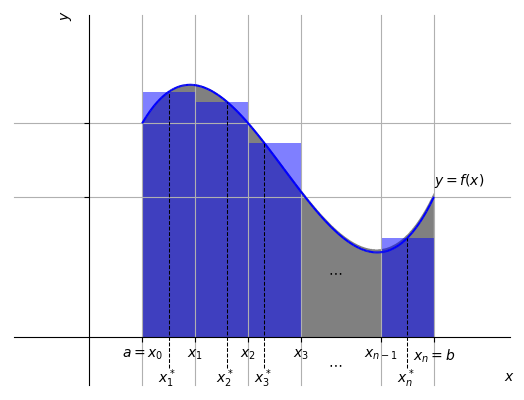
\includegraphics[width=0.9\textwidth]{./cap_int/dados/fig_soma_de_Riemann/fig_soma_de_Riemann}
  \caption{Ilustração da soma de Riemann.}
  \label{fig:soma_de_Riemann}
\end{figure}

\begin{obs}\normalfont{(Aproximação da área sob o gráfico)}
No caso de uma função não-negativa, uma soma de Riemann é uma aproximação da área sob seu gráfico e o eixo das abscissas\footnote{Veja o Exercício \ref{exer:int_geoRiemann} para uma interpretação geométrica no caso geral de funções contínuas.}. Veja a Figura \ref{fig:soma_de_Riemann}.
\end{obs}

\subsection{Integral definida}

A integral (definida) de $a$ até $b$ de uma dada função $f$ em relação a $x$ é denotada e definida por
\begin{equation}
  \int_a^b f(x)\,dx := \lim_{\|P\|\to 0} \sum_{i=1}^n f(x_i^*)\Delta x_i.
\end{equation}
De forma genérica, a integral definida de $a$ até $b$ é o limite das somas de Riemann quando a norma das partições $P$ do intervalo $[a, b]$ tendem a zero. Quando o limite existe, dizemos que $f$ é \emph{integrável} no intervalo $[a, b]$.

\begin{obs}
  Na notação de integral definida acima, chamamos $a$ de \emph{limite inferior} e $b$ de \emph{limite superior de integração}, $f$ é chamada de \emph{integrando} e $x$ de \emph{variável de integração}.
\end{obs}

\begin{obs}
  Funções contínuas são funções integráveis.
\end{obs}

\begin{figure}[H]
  \centering
  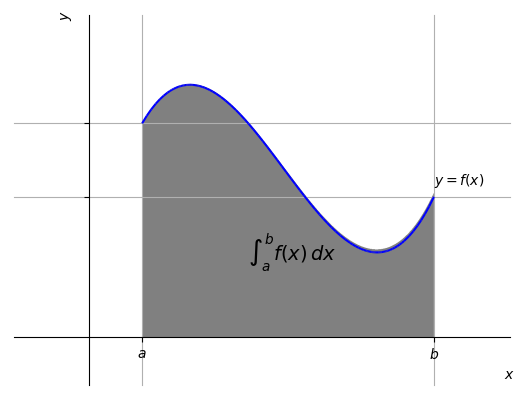
\includegraphics[width=0.9\textwidth]{./cap_int/dados/fig_geointdef/fig_geointdef}
  \caption{A integral definida como a área sob o gráfico.}
  \label{fig:geointdef}
\end{figure}

\begin{obs}\normalfont{(Área sob o gráfico)}\label{obs:int_area}
  No caso de uma função não-negativa,
  \begin{equation}
    \int_a^b f(x)\,dx
  \end{equation}
  é a área sob o gráfico de $f$\footnote{Veja o Exercício \ref{exer:int_geointdef} para uma interpretação geométrica no caso geral de funções contínuas.}. Veja a Figura \ref{fig:geointdef}.  
\end{obs}

\begin{ex}
  Vamos calcular
  \begin{equation}
    \int_0^1 1\,dx.
  \end{equation}
  Aqui, o integrando é a função constante $f(x) \equiv 1$ e o \emph{intervalo de integração} é $[a, b]$. Da Observação \ref{obs:int_area}, temos que esta integral é a área sob o gráfico de $f$ no intervalo $[0, 1]$. Esta área é um retângulo de altura $1$ e comprimento $1$. Logo,
  \begin{equation}
    \int_0^1 1\,dx = 1\cdot 1 = 1.
  \end{equation}
\end{ex}

\subsection*{Exercícios resolvidos}

\begin{exeresol}
  Calcule
  \begin{equation}
    \int_{-1}^1 \sqrt{1 - x^2}\,dx.
  \end{equation}
\end{exeresol}
\begin{resol}
  Esta integral corresponde à área sob o gráfico da função $f(x) = \sqrt{1 - x^2}$ restrita ao intervalo $[-1, 1]$. Observando que
  \begin{align}
    y = \sqrt{x^2 - 1} &\Rightarrow y^2 = 1 - x^2\\
                       &\Rightarrow y^2 + x^2 = 1,
  \end{align}
  vemos que esta é a área do semicírculo de raio $1$. Logo,
  \begin{equation}
    \int_{-1}^1 \sqrt{1 - x^2}\,dx = \frac{\pi \cdot 1^2}{2} = \frac{\pi}{2}.
  \end{equation}
\end{resol}

\begin{exeresol}
  Determine a função $F(x)$ tal que
  \begin{equation}
    F(x) = \int_0^x t\,dt,
  \end{equation}
  para todo $x\geq 0$. Então, mostre que $F'(x) = x$.
\end{exeresol}
\begin{resp}
  A integral definida
  \begin{equation}
    \int_0^x t\,dt
  \end{equation}
  é a área sob o gráfico de $f(t) = t$ restrita no intervalo $[0, x]$. Isto é, a área do triângulo retângulo de base $x$ e altura $x$. Logo,
  \begin{equation}
    F(x) = \int_0^x t\,dt = \frac{x\cdot x}{2} = \frac{x^2}{2}.
  \end{equation}
  Ou seja, temos $F(x) = x^2/2$ e, portanto,
  \begin{equation}
    F'(x) = \frac{1}{2}\cdot 2x = x.
  \end{equation}
\end{resp}

\subsection*{Exercícios}

\begin{exer}
  Calcule
  \begin{equation}
    \int_{-1}^2 2\,dx.
  \end{equation}
\end{exer}
\begin{resp}
  $6$
\end{resp}

\begin{exer}
  Calcule
  \begin{equation}
    \int_{-3}^{-1} 1-x\,dx.
  \end{equation}
\end{exer}
\begin{resp}
  $6$
\end{resp}

\begin{exer}
  Determine $F(x)$ tal que
  \begin{equation}
    F(x) = \int_{0}^{x} t+1\,dt.
  \end{equation}
  para $x\geq 0$. Então, calcule $F'(x)$.
\end{exer}
\begin{resp}
  $\displaystyle F(x) = \frac{x^2}{2} + x$; $F'(x) = x + 1$.
\end{resp}

\begin{exer}\label{exer:int_geoRiemann}
  Faça uma interpretação geométrica da uma soma de Riemann aplicada a uma função contínua e não positiva. Estenda sua interpretação para funções contínuas arbitrárias.
\end{exer}
\begin{resp}
  Dica: a soma de Riemann é uma aproximação da área líquida sob o gráfico da função.
\end{resp}

\begin{exer}\label{exer:int_geointdef}
  Faça uma interpretação geométrica de
  \begin{equation}
    \int_a^b f(x)\,dx
  \end{equation}
  quando $f$ é uma função contínua e não positiva. Estenda sua interpretação para funções contínuas arbitrárias.
\end{exer}
\begin{resp}
  Dica: $\displaystyle \int_a^b f(x)\,dx$é a área líquida sob o gráfico da função.
\end{resp}

\begin{exer}
  Calcule
  \begin{equation}
    \int_{-1}^2 -1\,dx.
  \end{equation}
\end{exer}
\begin{resp}
  $-3$
\end{resp}

\begin{exer}
  Calcule
  \begin{equation}
    \int_{-1}^{1} x\,dx.
  \end{equation}
\end{exer}
\begin{resp}
  $0$
\end{resp}

\section{Integral definida}

\emconstrucao

\subsection*{Exercícios resolvidos}

\emconstrucao

\subsection*{Exercícios}

\emconstrucao

\section{Integrais indefinidas}\label{cap_int_sec_intindef}

Seja $f(x)$ uma função. Dizemos que $F(x)$ é uma \emph{primitiva} de $f(x)$ quando
\begin{equation}
  F'(x) = f(x)
\end{equation}
para todo $x$ no domínio da $f$.

\begin{ex}\label{ex:primitiva}
  Seja $f(x) = 2x$. Notemos que $F(x) = x^2$ é uma primitiva de $f$, pois
  \begin{equation}
    F'(x) = 2x = f(x).
  \end{equation}
  Também, se $C$ é uma constante qualquer, $F(x) = x^2 + C$ é primitiva de $f(x)$. De fato, lembrando que a derivada de uma constante é zero, temos
  \begin{equation}
    F'(x) = 2x + 0 = 2x = f(x).
  \end{equation}
\end{ex}

\begin{obs}
  Se $F(x)$ é uma primitiva de $f(x)$, então $F(x)+C$, com $C$ constante, também é primitiva de $f(x)$.
\end{obs}

A \emph{integral indefinida} de uma função $f(x)$ é denotada por
\begin{equation}
  \int f(x)\,dx
\end{equation}
e é definida por
\begin{equation}
  \int f(x)\,dx = F(x) + C,
\end{equation}
onde $F(x)$ é uma primitiva de $f(x)$.

\begin{ex}
  Do observado no exemplo anterior (Exemplo \ref{ex:primitiva}), temos
  \begin{equation}
    \int 2x\,dx = x^2 + C.
  \end{equation}

  \ifispython
  Com o \verb+Sympy+, podemos computar a integral indefinida acima com o comando\footnote{Veja a Observação \ref{obs:cap_int_python}.}:
\begin{verbatim}
integrate(2*x)
\end{verbatim}
  \fi
  Observe que o \verb+Sympy+ não adiciona a constante indeterminada.
\end{ex}

\subsection{Regras básicas de integração}

Das regras básicas de derivação, podemos inferir as seguintes regras para integração:
\begin{itemize}
\item $\displaystyle \int 0\,dx = C$.
\item $\displaystyle \int 1\,dx = x + C$.
\item $\displaystyle \int af(x)\,dx = a\int f(x)\,dx$, $a\neq 0$ constante.
\item $\displaystyle \int f(x)\pm g(x)\,dx = \int f(x)\,dx \pm \int g(x)\,dx$.
\end{itemize}

\begin{ex}\label{ex:int_poli}
  \begin{align}
    \int x - 3x^2\,dx &= \int x\,dx - \int 3x^2\,dx\\
                      &= \int \frac{2}{2}x\,dx - x^3 + C\\
                      &= \frac{1}{2}\int 2x\,dx - x^3 + C\\
                      &= \frac{x^2}{2} - x^3 + C.
  \end{align}
\end{ex}

No exemplo anterior (Exemplo \ref{ex:int_poli}) integramos funções potências. Da regra de derivação
\begin{equation}
  [x^n]' = nx^{n-1}, \quad n\neq 0,
\end{equation}
temos
\begin{align}
  \int x^n\,dx &= \int \frac{n+1}{n+1}x^n\,dx, \quad n\neq -1,\\
               &= \frac{1}{n+1}\int (n+1)x^n\,dx,\\
               &= \frac{x^{n+1}}{n+1} + C.
\end{align}
Ou seja, obtemos a seguinte regra de integração para função potência
\begin{equation}
  \int x^n\,dx = \frac{x^{n+1}}{n+1} + C, \quad n\neq -1.
\end{equation}

\begin{ex}
  \begin{equation}
    \int 3x^{-2}\,dx = 3\int x^{-2}\,dx = 3\frac{x^{-2+1}}{-2+1} + C = -3x^{-1} + C = -\frac{3}{x} + C.
  \end{equation}
\end{ex}

Das regras de derivação para a função exponencial natural e logaritmo natural, temos
\begin{itemize}
\item $\displaystyle \int e^x\,dx = e^x + C$.
\item $\displaystyle \int \frac{1}{x}\,dx = \ln x + C$.
\end{itemize}
Também, como $(a^x)' = a^x\ln a$, temos
\begin{equation}
  \int a^x\,dx = \frac{a^x}{\ln a} + C.
\end{equation}

\subsection*{Exercícios resolvidos}

\emconstrucao

\subsection{Exercícios}

\emconstrucao

\section{Integração por substituição}\label{cap_int_sec_subs}

Seja $u = u(x)$. Usando de diferenciais, temos $du = u'(x)dx$. Logo,
\begin{equation}
  \int f(u(x))u'(x)\,dx = \int f(u)\,du.
\end{equation}
Esta é chamada de regra de integração por substituição.

\begin{ex}
  Consideremos
  \begin{equation}
    \int (2x+1)^2\,dx.
  \end{equation}
  Substituindo
  \begin{equation}
    u = 2x+1
  \end{equation}
  temos
  \begin{equation}
    du = 2dx.
  \end{equation}
  Portanto,
  \begin{align}
    \int (x+1)^2\,dx &= \int u^2\,\frac{du}{2}\\
                     &= \frac{1}{2}\int u^2\,du\\
                     &= \frac{1}{2}\frac{u^{2+1}}{2+1} + C\\
                     &= \frac{u^3}{6} + C\\
                     &= \frac{1}{6}(2x+1)^3 + C.
  \end{align}
\end{ex}

\subsection*{Exercícios resolvidos}

\begin{exeresol}
  Calcule
  \begin{equation}
    \int \frac{7}{(x-1)^2}\,dx.
  \end{equation}
\end{exeresol}
\begin{resol}
  Usamos a regra de integração por substituição
  \begin{equation}
    \int f(u(x))u'(x)\,dx = \int f(u)\,du.
  \end{equation}
  Escolhemos
  \begin{equation}
    u = x-1,
  \end{equation}
  e calculamos
  \begin{equation}
    \frac{du}{dx} = 1 \Rightarrow du = dx.
  \end{equation}
  Então, da fórmula, obtemos
  \begin{align}
    \int \frac{7}{(x-1)^2}\,dx &= \int \frac{7}{u^2}\,du\\
                               &= 7\int u^{-2}\,du\\
                               &= 7\frac{u^{-2+1}}{-2+1}\\
                               &= -\frac{7}{u}\\
                               &= \frac{7}{1-x}.
  \end{align}
\end{resol}

\emconstrucao

\subsection*{Exercícios}

\emconstrucao

\section{Integração por partes}\label{cap_int_sec_partes}

Sejam $u=u(x)$ e $v=v(x)$ funções diferenciáveis, então
\begin{equation}
  \frac{d}{dx}(uv) = \frac{du}{dx}v + u\frac{dv}{dx}.
\end{equation}
Integrando em ambos os lados, obtemos
\begin{equation}
  \int \frac{d (uv)}{dx}dx = \int \frac{du}{dx}vdx + \int u\frac{dv}{dx}dx,
\end{equation}
donde
\begin{equation}
  uv = \int vdu + \int udv.
\end{equation}
Daí, segue a \emph{fórmula de integração por partes}
\begin{equation}
  \int udv = uv - \int vdu.
\end{equation}

\begin{ex}
  Consideremos $\int xe^x\,dx$. Tomando
  \begin{align}
    &u = x \Rightarrow \frac{du}{dx} = 1 \Rightarrow du = dx,\\
    &dv = e^x\,dx \Rightarrow \int dv = \int e^x\,dx \Rightarrow v = e^x.
  \end{align}
  Então, da fórmula de integração por partes, temos
  \begin{align}
    \int xe^x\,dx &= \int udv = uv - \int vdu\\
                  &= xe^x - \int e^xdx\\
                  &= xe^x - e^x + C.
  \end{align}
\end{ex}

\subsection*{Exercícios resolvidos}

\begin{exeresol}
  Calcule
  \begin{equation}
    \int x\ln x\,dx.
  \end{equation}
\end{exeresol}
\begin{resol}
  Usamos a fórmula de integração por partes
  \begin{equation}
    \int udv = uv - \int vdu.
  \end{equation}
  Para tanto, escolhemos
  \begin{align}
    &u = \ln x \Rightarrow du = \frac{1}{x}\,dx\\
    &dv = x\,dx \Rightarrow v = \int x\,dx = \frac{x^2}{2}+C.
  \end{align}
  Tomando $C=0$, e usando a fórmula, obtemos
  \begin{align}
    \int x\ln x\,dx &= \int udv\\
                    &= uv - \int v\,du\\
                    &= \frac{x^2}{2}\ln x - \int \frac{x^2}{2}\frac{1}{x}\,dx\\
                    &= \frac{x^2}{2}\ln x - \frac{1}{2}\int x\,dx\\
                    &= \frac{x^2}{2}\ln x - \frac{1}{2}\frac{x^2}{2} + C\\
                    &= \frac{x^2}{2}\ln x - \frac{x^2}{4} + C.
  \end{align}

  \ifispython
  Podemos computar esta integral, usando o seguinte comando do \verb+Sympy+\footnote{Veja a Observação \ref{obs:cap_int_python}.}:
\begin{verbatim}
integrate(x*log(x),x)
\end{verbatim}
  \fi
\end{resol}

\emconstrucao

\subsection*{Exercícios}

\emconstrucao

\section{Integral definida}\label{cap_int_intdef}

\emconstrucao

\subsection{Teorema fundamental do cálculo}

O teorema fundamental do cálculo estabelece uma relação entre a integral definida de uma função e suas primitivas.

\begin{teo}\normalfont{(Teorema fundamental do cálculo)}
  Se $f$ é uma função contínua em um intervalo fechado $[a, b]$ e $F$ é qualquer primitiva de $f$ em $[a, b]$, então
  \begin{equation}
    \int_a^b f(x)\,dx = F(b)-F(a).
  \end{equation}
\end{teo}

\begin{obs}\label{obs:tfc1}
  Uma outra forma do teorema fundamental do cálculo é a seguinte: se $f$ é contínua em $[a, b]$, então
  \begin{equation}
    F(x) = \int_a^x f(t)\,dt
  \end{equation}
  é contínua em $[a, b]$, derivável em $(a, b)$ e sua derivada é
  \begin{equation}
    F'(x) = \frac{d}{dx}\int_a^x f(t)\,dt = f(x).
  \end{equation}
\end{obs}

\subsection{Substituição em integrais definidas}

Em algumas situações, faz-se necessário a aplicação da técnica de integração por substituição para integrais definidas. Neste contexto, sejam $f$ e $u$ funções dadas e $F$ uma primitiva de $f$. Então,
\begin{equation}
  [F(u)]' = F'(u)u' = f(u)u'.
\end{equation}
Portanto, pelo teorema fundamental do cálculo, temos
\begin{align}
  \int_a^b f(u(x))u'(x)\,dx &= F(u(x))|_{x=a}^{x=b}\\
                            &= F(u)|_{u=u(a)}^{u=u(b)}\\
                            &= \int_{u(a)}^{u(b)} f(u)\,du.
\end{align}
Resumidamente, temos que a \emph{regra da substituição em integrais definidas}, lê-se
\begin{equation}
  \int_a^b f(u(x))u'(x)\,dx = \int_{u(a)}^{u(b)} f(u)\,du.
\end{equation}

\subsection{Integração por partes para integrais definidas}

Podemos aplicar a fórmula de integração por partes para integrais definidas. Neste caso, temos
\begin{equation}
  \int_a^b f(x)g'(x)\,dx = f(x)g(x)|_{a}^b - \int_a^b g(x)f'(x)\,dx.
\end{equation}

\subsection*{Exercícios resolvidos}

\begin{exeresol}
  Calcule
  \begin{equation}
    \int_0^1x\sqrt{1-x^2}\,dx.
  \end{equation}
\end{exeresol}
\begin{resol}
  Vejamos as seguintes formas de calcular esta integral definida.
  \begin{itemize}
  \item Solução 1: aplicando a regra de substituição em integrais definidas.
    \begin{equation}
      \int_a^bf(u(x))u'(x)\,dx = \int_{u(a)}^{u(b)} f(u)\,du.
    \end{equation}
    Escolhendo, $u = 1-x^2$, temos $du = -2x\,dx$. Daí, segue
    \begin{align}
      \int_0^1x\sqrt{1-x^2}\,dx &= \int_{u(0)}^{u(1)}x\sqrt{u}\,\frac{du}{-2x}\\
                                &= -\frac{1}{2}\int_{1}^0 u^{\frac{1}{2}}\,du\\
                                &= -\frac{1}{2}\left.\frac{u^{\frac{1}{2}+1}}{\frac{1}{2}+1}\right|_{u=1}^0\\
                                &= -\frac{1}{3}\left.\sqrt{u^3}\right|_{u=1}^0\\
                                &= \frac{1}{3}.
    \end{align}
  \item Solução 2: calculando uma primitiva em função de $x$.
    Para obtermos uma primitiva em função de $x$, calculamos a integral indefinida
    \begin{equation}
      \int x\sqrt{1-x^2}\,dx.
    \end{equation}
    Como anteriormente, usamos a regra de substituição. Escolhendo $u=1-x^2$, temos $du = -2x\,dx$ e, portanto
    \begin{align}
      \int x\sqrt{1-x^2}\,dx &= \int x\sqrt{u}\,\frac{du}{-2x}\\
                             &= -\frac{1}{2}\int u^{\frac{1}{2}}\,du\\
                             &= -\frac{1}{2}\frac{u^{\frac{1}{2}+1}}{\frac{1}{2}+1}\\
                             &= -\frac{1}{3}\sqrt{u^3}\\
                             &= -\frac{1}{3}\sqrt{(1-x^2)^3} + C.
    \end{align}
    Então, do teorema fundamental do cálculo, temos
    \begin{equation}
      \int_0^1 x\sqrt{1-x^2}\,dx = -\frac{1}{3}\left.\sqrt{(1-x^2)^3}\right|_{0}^1 = \frac{1}{3}.
    \end{equation}
  \end{itemize}

  \ifispython
  Para computarmos esta integral definida, podemos usar o seguinte comando do \verb+Sympy+:
\begin{verbatim}
integrate(x*sqrt(1-x**2),(x,0,1))
\end{verbatim}
  \fi
\end{resol}

\begin{exeresol}
  Calcule
  \begin{equation}
    \int_{-1}^1 xe^x\,dx.
  \end{equation}
\end{exeresol}
\begin{resol}
  Vamos usar a fórmula de integração por partes para integrais definidadas
  \begin{equation}
    \int_a^b f(x)g'(x)\,dx = f(x)g(x)|_{a}^b - \int g(x)f'(x)\,dx.
  \end{equation}
  Para tanto, escolhemos $f(x) = x$ e $g'(x) = e^x$, donde
  \begin{equation}
    f'(x) = 1,\quad\text{e}\quad g(x) = \int g'(x)\,dx = \int e^x\,dx = e^x + C.
  \end{equation}
  Escolhendo $C=0$ e usando a fórmula, temos
  \begin{align}
    \int_{-1}^1 xe^x\,dx &= \int_{-1}^1 f(x)g'(x)\,dx\\
                         &= f(x)g(x)|_{-1}^1 - \int_{-1}^1 g(x)f'(x)\,dx\\
                         &= xe^x|_{-1}^1 - \int_{-1}^1 e^x\,dx\\
                         &= e+e^{-1}-[e^x]_{-1}^1\\
                         &= e+e^{-1}-(e-e^{-1})\\
                         &= 2e^{-1}.
  \end{align}
  \ifispython
  Para computarmos esta integral definida, podemos usar o seguinte comando do \verb+Sympy+:
\begin{verbatim}
integrate(x*exp(x),(x,-1,1))
\end{verbatim}
  \fi
\end{resol}

\emconstrucao

\subsection*{Exercícios}

\begin{exer}
  Calcule
  \begin{equation}
    \int \frac{7}{(x-1)^2}\,dx.
  \end{equation}
\end{exer}
\begin{resp}
  $\frac{7}{2}$
\end{resp}

\begin{exer}
  Calcule
  \begin{equation}
    \int_0^{\ln 3} e^{2x}\,dx.
  \end{equation}
\end{exer}
\begin{resp}
  $4$
\end{resp}

\begin{exer}
  Calcule
  \begin{equation}
    \int_0^{\sqrt{e-1}} \frac{x}{x^2+1}\,dx.
  \end{equation}
\end{exer}
\begin{resp}
  $\frac{1}{2}$
\end{resp}

\begin{exer}
  Calcule
  \begin{equation}
    \int_{-1}^1 x^2e^x\,dx.
  \end{equation}
\end{exer}
\begin{resp}
  $-\frac{5}{e}+e$
\end{resp}

